\section{Hardware Setup/implementation}
\subsection{System Architecture}

\begin{figure}[h]
  \centering
  \includegraphics[width=1\textwidth]{fig/system}
  \caption{System architecture}
  \label{fig:system}
\end{figure}

The overall system architecture is illustrated in Figure \ref{fig:system}. 

\subsection{System Setup}
Figure \ref{fig:setup_n} and \ref{fig:setup_d} shows the complete system in a picture of how the hardware is connected for normal operation and for debugging.

\begin{figure}[H]
  \centering
  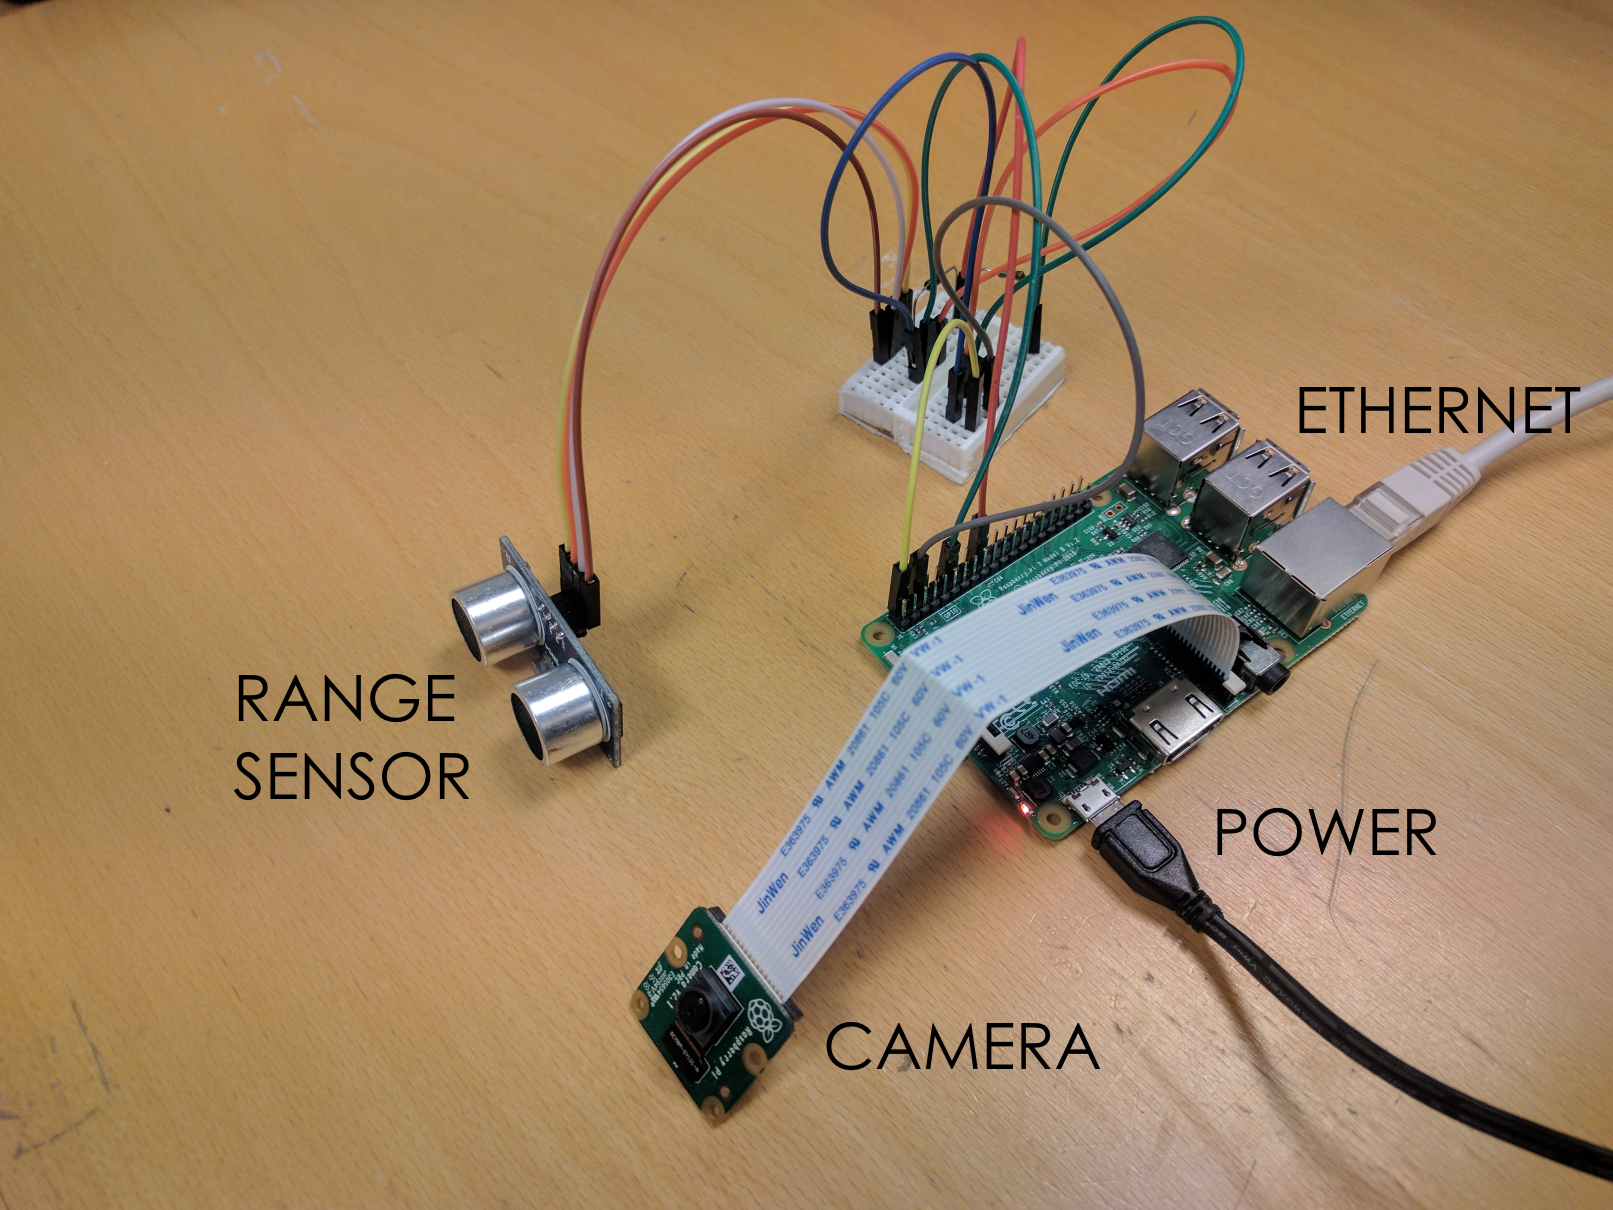
\includegraphics[width=0.6\textwidth]{fig/setup_normal}
  \caption{Normal hardware setup}
  \label{fig:setup_n}
\end{figure}
\begin{figure}[H]
  \centering
  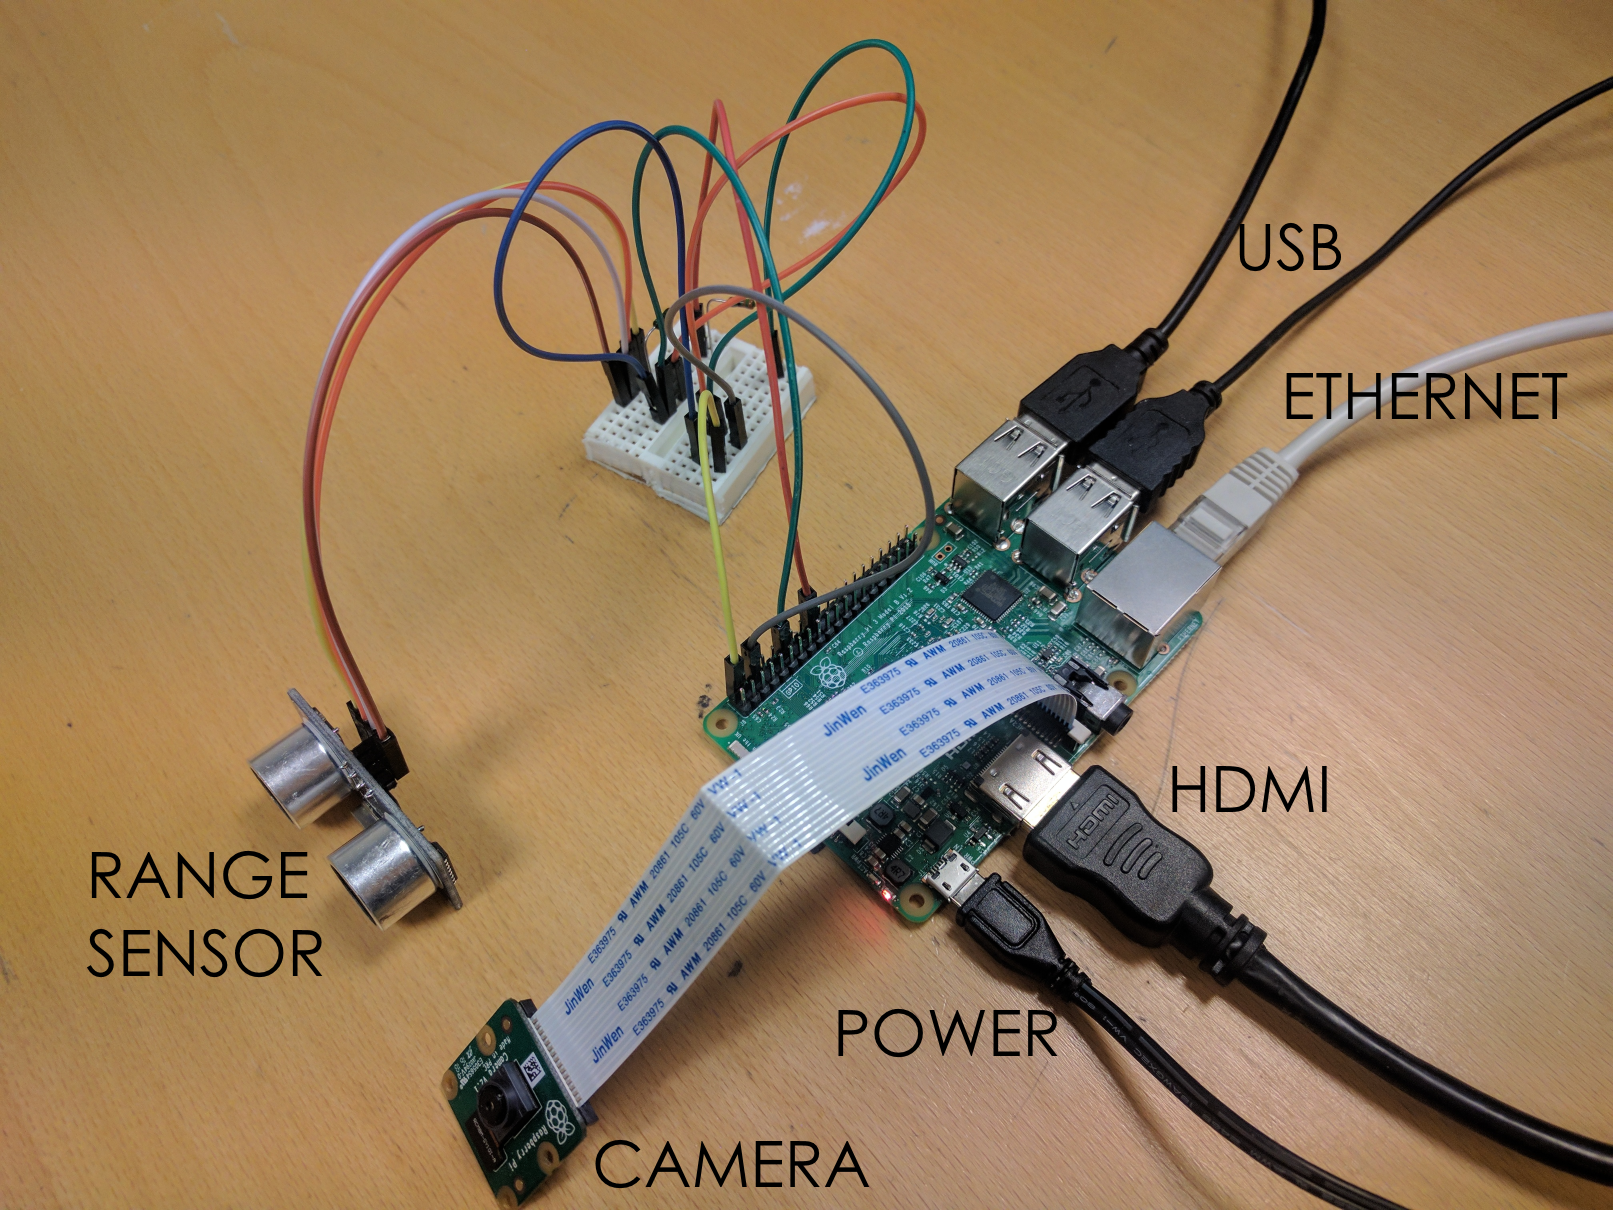
\includegraphics[width=0.6\textwidth]{fig/setup_debug}
  \caption{Debug hardware setup}
  \label{fig:setup_d}
\end{figure}

\subsection{Raspberry Pi}

\begin{figure}[H]
  \centering
  \includegraphics[width=1\textwidth]{fig/pi3}
  \caption{Raspberry Pi 3 Model B. \cite{pi3}}
  \label{fig:pi3}
\end{figure}

Figure \ref{fig:pi3} displays most of the I/O interfaces on the Raspberry Pi 3 Model B.

\begin{figure}[H]
  \centering
  \includegraphics[width=1\textwidth]{fig/gpio}
  \caption{GPIO Pins on the Raspberry Pi 3\cite{rpi}}
  \label{fig:gpio}
\end{figure}

Figure \ref{fig:gpio} details the GPIO pins on the Raspberry Pi 

\subsection{Camera}
\subsection{Range sensor}
The HC-SR04 is a very easy sensor to use, but in order to make it compatible with the Raspberry Pi, there are some modifications needed. The GPIO input pins on the Raspberry Pi is made for 3.3V while the ECHO output pin on the HC-SR04 delivers 5V. So in order for the Raspberry Pi to interact with the HC-SR04, I need to reduce the voltage to 3.3V.\\

\begin{figure}[h]
  \centering
  \includegraphics[width=0.3\textwidth]{fig/volt}
  \caption{Voltage divider}
  \label{fig:volt}
\end{figure}

This can be done with a simple voltage divider. Figure \ref{fig:volt} illustrates a simple voltage divider circuit that can be easily created with two resistors since we know the input and output voltages. The formula for a voltage divider is as follows:

\begin{align}
V_{out} = V_{in}\times \frac{R_2}{R_1 + R_2}
\end{align}

I want the $V_{out}$ to be 3.3V, and the $V_{in}$ is 5V. By a combination of resistors R1 and R2 the desired output voltage can be obtained. By picking R1$ = 820\Omega$ and R2$ = 1500\Omega$ we get:

\begin{align*}
V_{out} = 5 \times \frac{1500}{820+1500} = 3.23 V
\end{align*}

This is close enough for our application, and this is verified in the tests later in the thesis. Figure \ref{fig:rangesensor} shows how this voltage divider is implemented, and to which GPIO pins on the Raspberry Pi it is connected.

\begin{figure}[h]
  \centering
  \includegraphics[width=0.4\textwidth]{fig/SensorSketch}
  \caption{Range sensor setup}
  \label{fig:rangesensor}
\end{figure}
